\section{Things brought by Good Practice in UserPackage}
	
		\begin{frame}
			\frametitle{Things brought by extra}
			
			contenu...
		\end{frame}
		
		\begin{frame}
			\frametitle{nTheorem}
			
			The interactions beteween ntheorem and beamer has been solved.
			
			\begin{theorem}
				contenu...
			\end{theorem}
			
			\begin{proof}
				contenu...
			\end{proof}
		\end{frame}	
		
		\begin{frame}
			\frametitle{Glossaries}
			
			Here is an example of acronym using glossaries: \gls{lbm}
			
			And an example of equation in colors, the Boltzmann equation:
			\begin{equation}
				{\color{blue} \partial_t \gls{BoltzDist}(x,\xi,t)} + {\color{red} \xi\cdot\partial_x \gls{BoltzDist}(x,\xi,t)} + {\color{green!60!black!80} g\cdot\partial_\xi f(x,\xi,t)}
				= {\color{yellow!80!orange!85!black} \Omega(\gls{BoltzDist},\gls{BoltzDist})}
			\end{equation}
			where $\gls{BoltzDist}$ is a variable defined through glossaries.
			
		\end{frame}
		
		\begin{frame}[fragile]
			\frametitle{Cite in the footnote}
			
			Some text that requires a reference\footfullciteBeamer{knuth92}. 
			Using the command\footnote{Please note that this command can be used slide-by-slide the command footnote.}
			\begin{verbatim}			
					\footfullciteBeamer{<bibKey>}
			\end{verbatim}
			
			The command to cite in text mode is also possible with 
			\begin{verbatim}			
					\fullciteBeamer{<bibKey>}
			\end{verbatim}
			and giving \fullciteBeamer{ConcreteMath}
		\end{frame}
		
		\begin{frame}%[fragile]
			\frametitle{Video}
			
			The last but not least feature present is a macro simplifying the way to include videos in beamer presentation. 
			
			It requires to define the OS on which the pdf will be red, thanks to the command 
			
			Then, the video can be included with the command 
%			\begin{verbatim}			
%				\def\OSvar{windows}
%			\end{verbatim}
%			voila
			\includeVideo[% no space
					width=0.3\linewidth, height=0.2\linewidth,
				]% Options
				{\PathS/Air_convec.mp4}% Video File
				{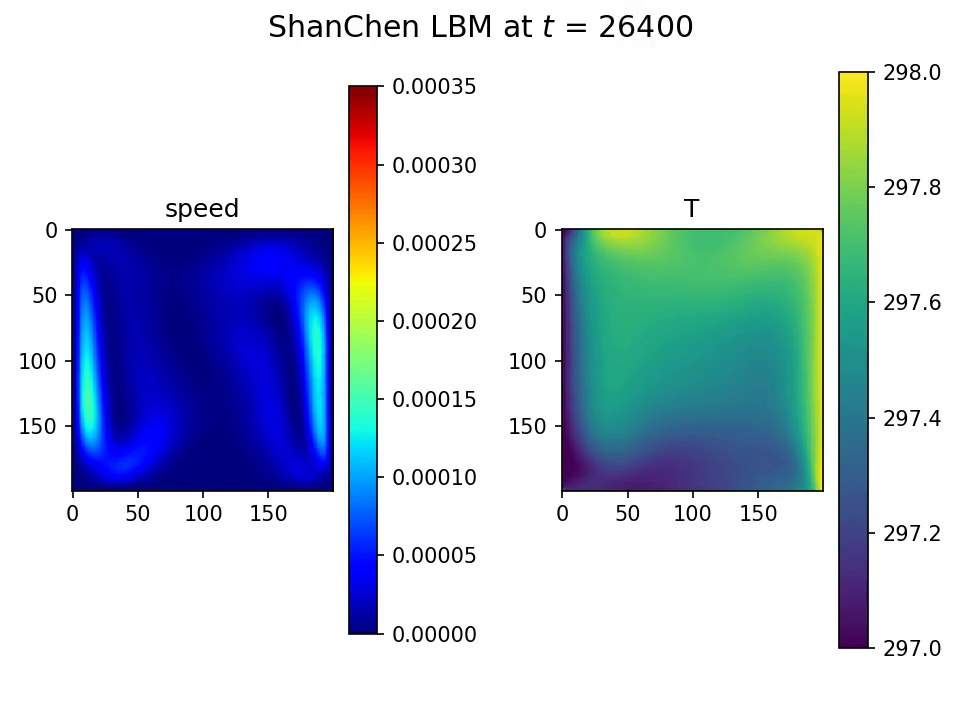
\includegraphics[width=0.3\linewidth,height=0.2\linewidth]{\PathS/Thermal_convec.png}}
		\end{frame}	
		
		\newcounter{r}
		\newcommand{\escalar}[1]{
		\setcounter{r}{#1 * #1 * #1}
		}
		%
		\newcounter{m}
		\setcounter{m}{0}
		\newcounter{mc}
		%
		\begin{frame}[fragile]{Animated Integral}
			\begin{center}
			\begin{animateinline}[loop, poster = first, controls, palindrome]{2}
				\whiledo{\them < 21}{
			   \begin{tikzpicture}[scale=1.25]
				   \draw[red,thick,<->] (-1,1) parabola bend (0,0) (2.1,4.41)
				       node[below right] {$y=x^2$};
				   \draw[loosely dotted] (-1,0) grid (4,4);
				   %\path[use as bounding box] (-2,-1) rectangle (5,5);
				   \draw[->] (-0.2,0) -- (4.25,0) node[right] {$x$};
				   \draw[->] (0,-0.25) -- (0,4.25) node[above] {$y$};
				   \foreach \x/\xtext in {1/1, 2/2, 3/3}
				   \draw[shift={(\x,0)}] (0pt,2pt) -- (0pt,-2pt) node[below] {$\xtext$};
				   \foreach \y/\ytext in {1/1, 2/2, 3/3, 4/4}
				   \draw[shift={(0,\y)}] (2pt,0pt) -- (-2pt,0pt) node[left] {$\ytext$};
					%
				   \setcounter{mc}{\value{m}*\value{m}}
				   \shade[top color=blue,bottom color=gray!50]
				       (0,0) parabola (0.1*\them,0.01*\themc) |- (0,0);
				   \escalar{\them}
				   \draw (3cm,2pt) node[above]
				       {$\displaystyle\int\limits_0^{\them/10} \!\!x^2\mathrm{d}x = 
				           \displaystyle\frac{\ther}{3000}$};
				   \draw[fill=orange,color=orange] (0.1*\them,0.01*\themc) circle (0.5pt);
			   \end{tikzpicture}
			   %
			   \stepcounter{m}
			   \ifthenelse{\them < 21}{
			           \newframe
			   }{
		   \end{animateinline}\relax % BREAK
		   }
			} % END \whiledo...
			\end{center}
		\end{frame}